\begin{figure*}[tb!]
\begin{subfigure}[t]{.33\textwidth}
  \centering
   \captionsetup{width=.9\linewidth}
    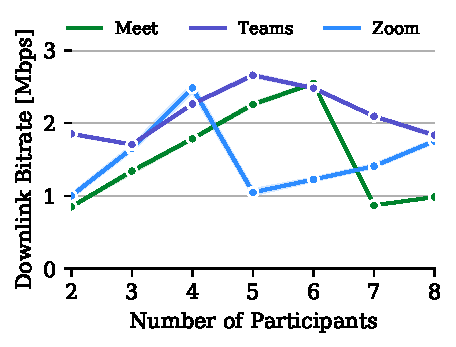
\includegraphics[width=1\textwidth,keepaspectratio]{../figures/modality/speaker_recv.pdf}
    \caption{Downlink traffic of client whose video is viewed in gallery mode}
    \label{fig:gallery-recv}
\end{subfigure}
\hfill
\begin{subfigure}[t]{.33\textwidth}
  \centering
   \captionsetup{width=.9\linewidth}
    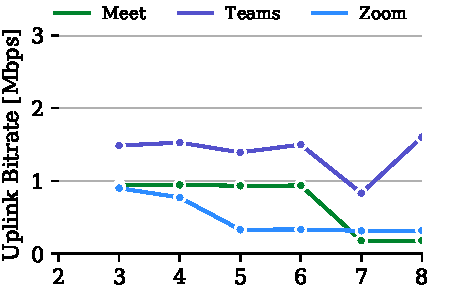
\includegraphics[width=1\textwidth,keepaspectratio]{../figures/modality/gallery_send.pdf}
    \caption{Uplink traffic of client whose video is viewed in gallery mode}
    \label{fig:gallery-send}
\end{subfigure}
\hfill
\begin{subfigure}[t]{.33\textwidth}
  \centering
   \captionsetup{width=.9\linewidth}
    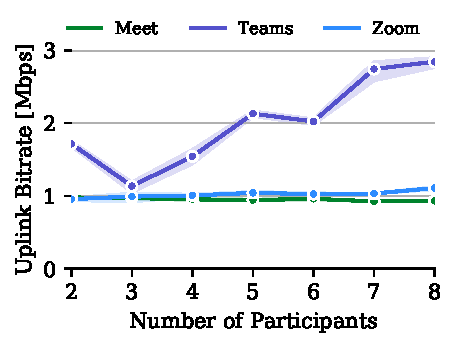
\includegraphics[width=1\textwidth,keepaspectratio]{../figures/modality/speaker_send.pdf}
    \caption{Uplink traffic of client whose video is pinned by all other participants (speaker mode)}
    \label{fig:speaker-send}
\end{subfigure}
\caption{Network utilization in different viewing modes. The bands represent 90\% confidence intervals.}
\label{fig:viewing-mode}
\end{figure*}




\section{Call Modalities}\label{sec:usage_modality}

People now increasingly rely on video conferencing for remote work,
school, and even large virtual conferences (such as this one!),
particularly during the COVID-19 pandemic, which has shifted many in-person
activities to virtual forums. These settings involve many
participants, which raises questions concerning performance and network
utilization of VCAs in settings involving multiple users.
We study network utilization under two prominent call modalities: 
\begin{enumerate}
    \itemsep=-1pt
    \item the
    number of participants in a call and 
\item the viewing mode.
\end{enumerate}
\noindent
We consider two
viewing modes that are common across all three VCAs: \textit{speaker} mode
wherein a specific user's video is pinned on the call and \textit{gallery}
mode, in which all participants' video are shown on the screen.  Each
experiment consists of a 2-minute call with $n$ users and specific viewing
mode. We vary the number of clients in the call from two to eight, across both
gallery and speaker modes.
We perform five experiment for each (number, viewing mode) combination; we log the
network utilization of Client C1 for each call.  Although it is
difficult to evaluate these applications for hundreds of simultaneous users,
we can nevertheless explore trends in utilization and performance for a
smaller number of users and observe various utilization trends. Larger-scale
experiments could be a possible area for future work.


\subsection{Number of Users}

To explore the effect of the number of users on utilization, we fix the
viewing mode to \textit{gallery}, which is the default viewing mode in all of
the VCAs. Figures~\ref{fig:gallery-recv} and~\ref{fig:gallery-send} show the
average downstream and upstream network utilization respectively for different
numbers of participants.  Total downstream utilization depends on both the
number of video streams and the data rate of each stream.  Utilization in both
directions typically {\em decreases} as the number of participants increases
in a \meet or \zoom call. In the case of \zoom, the uplink utilization drops
from 0.8~Mbps to 0.4~Mbps as number of participants increases from 4 to 5. For \meet, the reduction happens at n = 7, from
1~Mbps to 0.2~Mbps.  Both \meet and \zoom have tiled-screen display with each
user displayed in a separate tile.  As the number of users increases, the tile
size shrinks to accommodate all the users on the fixed size screen. For instance, \zoom uses a 2$\times$2 grid for 4 participants; switching to 5 participants creates a third row of video feeds making each individual video feed smaller.  The
sender uses this opportunity to reduce the resolution of transmitted video,
leading to reduction in upstream utilization.

We observe a similar reduction in downstream utilization at 5 and 7
participants for \zoom and \meet, respectively
(Figure~\ref{fig:gallery-recv}). However, there are also notable differences
when compared to the uplink utilization. For instance, the downlink
utilization for Google Meet increases from 1.25 Mbps to 2.5 Mbps when the
number of participants increases from 3 to 6, while upstream utilization stays
mostly constant. The trend is similar for \zoom as the number of participants
increases beyond than 5. 

\teams does not exhibit these trends: upstream utilization remains almost
constant as the number of participants changes. Downstream utilization
increases until five participants and drops as more participants join the call.
\teams has a fixed 4-tile layout on Linux. It thus displays
only a {\em subset} of participants if a call has more than four participants
which
may explain why the sending rate does not change, particularly as the number
of videos and the frame size may not
change significantly with more users. It is, however, not clear why the
downstream utilization decreases in calls with more than participants; this
phenomenon deserves more exploration. 

\subsection{Viewing Mode}

For all three VCAs, viewing a user's video in speaker mode leads to greater
uplink consumption on {\em that} user's network as compared to gallery mode.
Putting C1 on the speaker mode enlarges its tile size on other users' screen.
The sender streams the video at a high resolution to provide a high better user experience,
thus leading to increase in uplink utilization compared to when C1
was not pinned by other users. \zoom and \meet consistently send at 1 Mbps
when all clients pin C1's video, regardless of the number of participants.
Note that, only one client needed to put C1 on speaker for this behavior. Each
client can decide to pin any client independently of others.

The behavior of \teams differs from \meet and \zoom in this regard, as well.
C1's uplink utilization continues to increase from 1.25 Mbps with 3
participants to 2.9 Mbps participants when it is put on speaker mode. We
checked if the increase could be attributed to \teams communicating with
multiple destinations (e.g., with each user separately). However, we observe
that all of the traffic was directed to a single server. It is not clear what
contributes to the increase in traffic for \teams but this clearly leads to
inefficient network utilization, especially when compared to \zoom and \meet. 
\vspace{5pt}
\begin{mdframed}[roundcorner=5pt, backgroundcolor=black!10]
    \paragraph{Takeaways}: Each participant's video layout affects client's
    network utilization. Calls with more participants can {\em decrease} upstream and downstream utilization 
    for each participant, depending on how the VCA displays participant video.
    The settings of one participant (e.g., pinning a video, using speaker mode
    vs. gallery mode) can also affect the upstream utilization of {\em other}
    participants.
\end{mdframed}

